\documentclass{ximera}

\newcommand{\RR}{\mathbb R}
\renewcommand{\d}{\,d}
\newcommand{\dd}[2][]{\frac{d #1}{d #2}}
\renewcommand{\l}{\ell}
\newcommand{\ddx}{\frac{d}{dx}}
\newcommand{\dfn}{\textbf}
\newcommand{\eval}[1]{\bigg[ #1 \bigg]}


\author{Bart Snapp \and Jim Talamo}

\outcome{Compute directional derivatives.}
\outcome{Use the directional derivative to show that the gradient vector points in the initial direction of greatest increase for the function.}

\title[Dig-In:]{The directional derivative}

\begin{document}
\begin{abstract}
  We introduce a way of analyzing the rate of change in a given
  direction.
\end{abstract}
\maketitle

One way to think about partial derivatives is as follows: Given a
differentiable function $F:\R^2\to\R$,
\begin{itemize}
  \item $\pp[F]{x}$ gives the rate of change of $F$ in the $\veci$
    direction.
  \item $\pp[F]{y}$ gives the rate of change of $F$ in the $\vecj$
    direction.
\end{itemize}

Thus if we want to know the rate of change in \textit{any} direction, we could use the scalar projection:
\[
\scal_\uvec{u} \vector{\pp[F]{x},\pp[F]{y}} = \grad F(x,y) \dotp \uvec{u}
\]
this will give the rate of change of $F$ in the direction $\uvec{u}$.
This is a new type of derivative called the directional derivative.
\begin{definition}
  The \dfn{directional derivative} is computed by
  \[
  D_\uvec{u}(F) = \grad F(\vec{x})\dotp \uvec{u}
  \]
  where $\uvec{u}$ is a unit vector.
\end{definition}
The directional derivative tells us how $F$ changes if we move some
direction. If we want to make $D_\uvec{u}(F)$ as large as possible, it
makes sense to let $\uvec{u}$ be the direction of gradient since the
dot product
\[
\grad F(\vec{x})\dotp \uvec{u}
\]
is largest when $\uvec{u}$ is in the same direction as $\grad F$.

This tells us something very important about the gradient vector:

\begin{quote}
Given a function $F:\R^n\to\R$ \textbf{the gradient vector points in the
initial direction of greatest increase} for $F$.
\end{quote}
\begin{onlineOnly}
  We can see this in the interactive below. 
  \begin{center}
    \geogebra{wd5mrudh}{800}{600} %https://ggbm.at/wd5mrudh
  \end{center}
  The gradient at each point is a vector pointing in the
  $(x,y)$-plane. The direction of the vector tells us which initial
  direction to leave a point in the $(x,y)$-plane in order to find the
  greatest increase for $F$.
\end{onlineOnly}




\begin{example}
  Let
  \[
  F(x,y) = -x^2+2x-y^2+2y+1.
  \]
  Compute and interpret $\grad F(1,1)$.
  \begin{explanation}
    Write with me
    \[
    \grad F(x,y) = \vector{\answer[given]{-2x+2},\answer[given]{-2y+2}}.
    \]
    However, we see $\grad F(1,1) =
    \vector{\answer[given]{0},\answer[given]{0}}$. Since there is no
    initial direction of greatest increase, we must be at a local
    maximum for the function. Indeed we are, behold:
    \begin{image}
      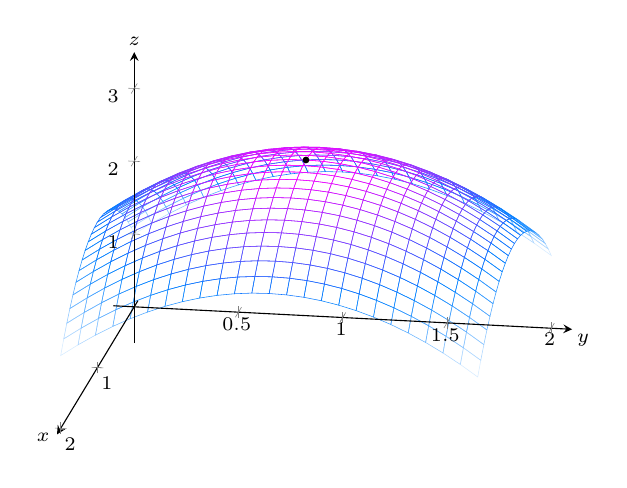
\begin{tikzpicture}
        \begin{axis}%
          [tick label style={font=\scriptsize},axis on top,
	    axis lines=center,
	    view={100}{25},
	    name=myplot,
	    %xtick=\empty,
	    %ytick={5},
	    %ztick={.7,-.7},
	    minor xtick=1,
	    minor ytick=1,
	    ymin=-.1,ymax=2.1,
	    xmin=-.1,xmax=2.1,
	    zmin=-.5, zmax=3.5,
	    every axis x label/.style={at={(axis cs:\pgfkeysvalueof{/pgfplots/xmax},0,0)},xshift=-5pt,yshift=-1pt},
	    xlabel={\scriptsize $x$},
	    every axis y label/.style={at={(axis cs:0,\pgfkeysvalueof{/pgfplots/ymax},0)},xshift=4pt,yshift=-4pt},
	    ylabel={\scriptsize $y$},
	    every axis z label/.style={at={(axis cs:0,0,\pgfkeysvalueof{/pgfplots/zmax})},xshift=0pt,yshift=4pt},
	    zlabel={\scriptsize $z$},
            colormap/cool
	  ]
          
          \addplot3[domain=0:2,,y domain=0:2,
            mesh,samples=25,samples y=25,very thin,z buffer=sort] {-x^2-y^2+2*x+2*y+1};
          \filldraw [black,] (axis cs:1,1,3) circle (1pt);
        \end{axis}
      \end{tikzpicture}
    \end{image}
    Ah! The point $(1,1)$ lies at the top of a paraboloid. In all
    directions, the instantaneous rate of change is $0$.
  \end{explanation}
\end{example}


\end{document}
